\documentclass{MYsig-alternate}
%  \documentclass{acm_proc_article-sp}
\usepackage{algorithm}
\usepackage{url}
\usepackage[noend]{algorithmic}
\usepackage{amsmath}
\usepackage{amsfonts}
\usepackage{amssymb}
\usepackage{color}
\usepackage{subfig}

\DeclareCaptionType{copyrightbox}

\def\BibTeX{Bib\TeX}
\parindent=0pt
\parskip=\baselineskip

% Please leave SVN version number $Revision: 453 $
% Remember to enter the SVN command 
%      svn propset svn:keywords "Revision" thisFile.tex


\begin{document}

\title{Instance-Based Parameter Tuning\\
for Evolutionary AI Planning}


 \numberofauthors{2}
 
 \author{
 \alignauthor
 M{\'a}ty{\'a}s Brendel\\
        \affaddr{Projet TAO, INRIA Saclay \& LRI}\\
        \affaddr{Universit{\'e} Paris Sud}\\
        \affaddr{Orsay, France}\\
        \email{matthias.brendel@lri.fr}
 \alignauthor
 Marc Schoenauer\\
        \affaddr{Projet TAO, INRIA Saclay \& LRI}\\
        \affaddr{Universit{\'e} Paris Sud}\\
        \affaddr{Orsay, France}\\
        \email{marc.schoenauer@inria.fr}
 }

\date{February 9, 2011}
\maketitle
\begin{abstract}
 \noindent Learn-and-Optimize ~(LaO) ~is ~a ~generic ~surrogate ~based method for parameter tuning combining learning and optimization. In this paper LaO is used to tune Divide-and-Evolve (DaE), an Evolutionary Algorithm for AI Planning. The LaO framework makes it possible to learn the relation between some features describing a given instance and the optimal parameters for this instance, thus it enables to extrapolate to unknown instances in the same domain. Moreover, the learned model is used as a surrogate-model to accelerate the search for the optimal parameters. The proposed implementation of LaO uses an Artificial Neural Network for learning the mapping between features and optimal parameters, and the Covariance Matrix Adaptation Evolution Strategy for optimization. Results demonstrate that LaO is capable of improving the quality of the DaE results even with only a few iterations. The main limitation of the DaE case-study is the limited learning time and amount of meaningful features that are available. However, it is demonstrated that the learned model is capable of generalization in the domain to unknown instances. 

\end{abstract}

\category{I.2.6}{Computing Methodologies}{Artificial Intelligence }{Learning} {Parameter learning}

\terms{Theory}

\keywords{parameter tuning, AI Planning, evolutionary algorithms} % NOT required for Proceedings


\section{Introduction}

All state of the art parameter tuning techniques, like for example F-Race, REVAC and ParamILS \cite{Montero:2010} face the same crucial generalization issue: the generalization of a parameter-set that has been optimized for a given problem to another one. The answer of course depends on the similarity of the problems. However, in AI Planning, sufficiently accurate features have not been specified that would allow to describe the problem, no design of a general learning framework has been proposed, and no general experiments have been carried out. This paper makes a step toward a framework for parameter tuning applied generally for AI Planning and proposes a preliminary set of features. The Learn-and-Optimize (LaO) framework consists of the combination of optimizing and learning, i.e., finding the mapping between features and best parameters.

In this paper, the target optimization technique is Evolutionary Algorithms (EA), more precisely the evolutionary AI planner called Divide-and-Evolve (DaE). However, DaE will be here considered as a black-box algorithm as described in \cite{BibEvoCop:2010}. 

\section{Learn-and-Optimize}
\label{section:LaO}

As \cite{BibGECCO:2010} demonstrates parameters tuned for one instance may not be optimal for other instances. One workaround is to aim at learning a complex relation between instances and optimal parameters.

\begin{figure}[h!]
  \centering
    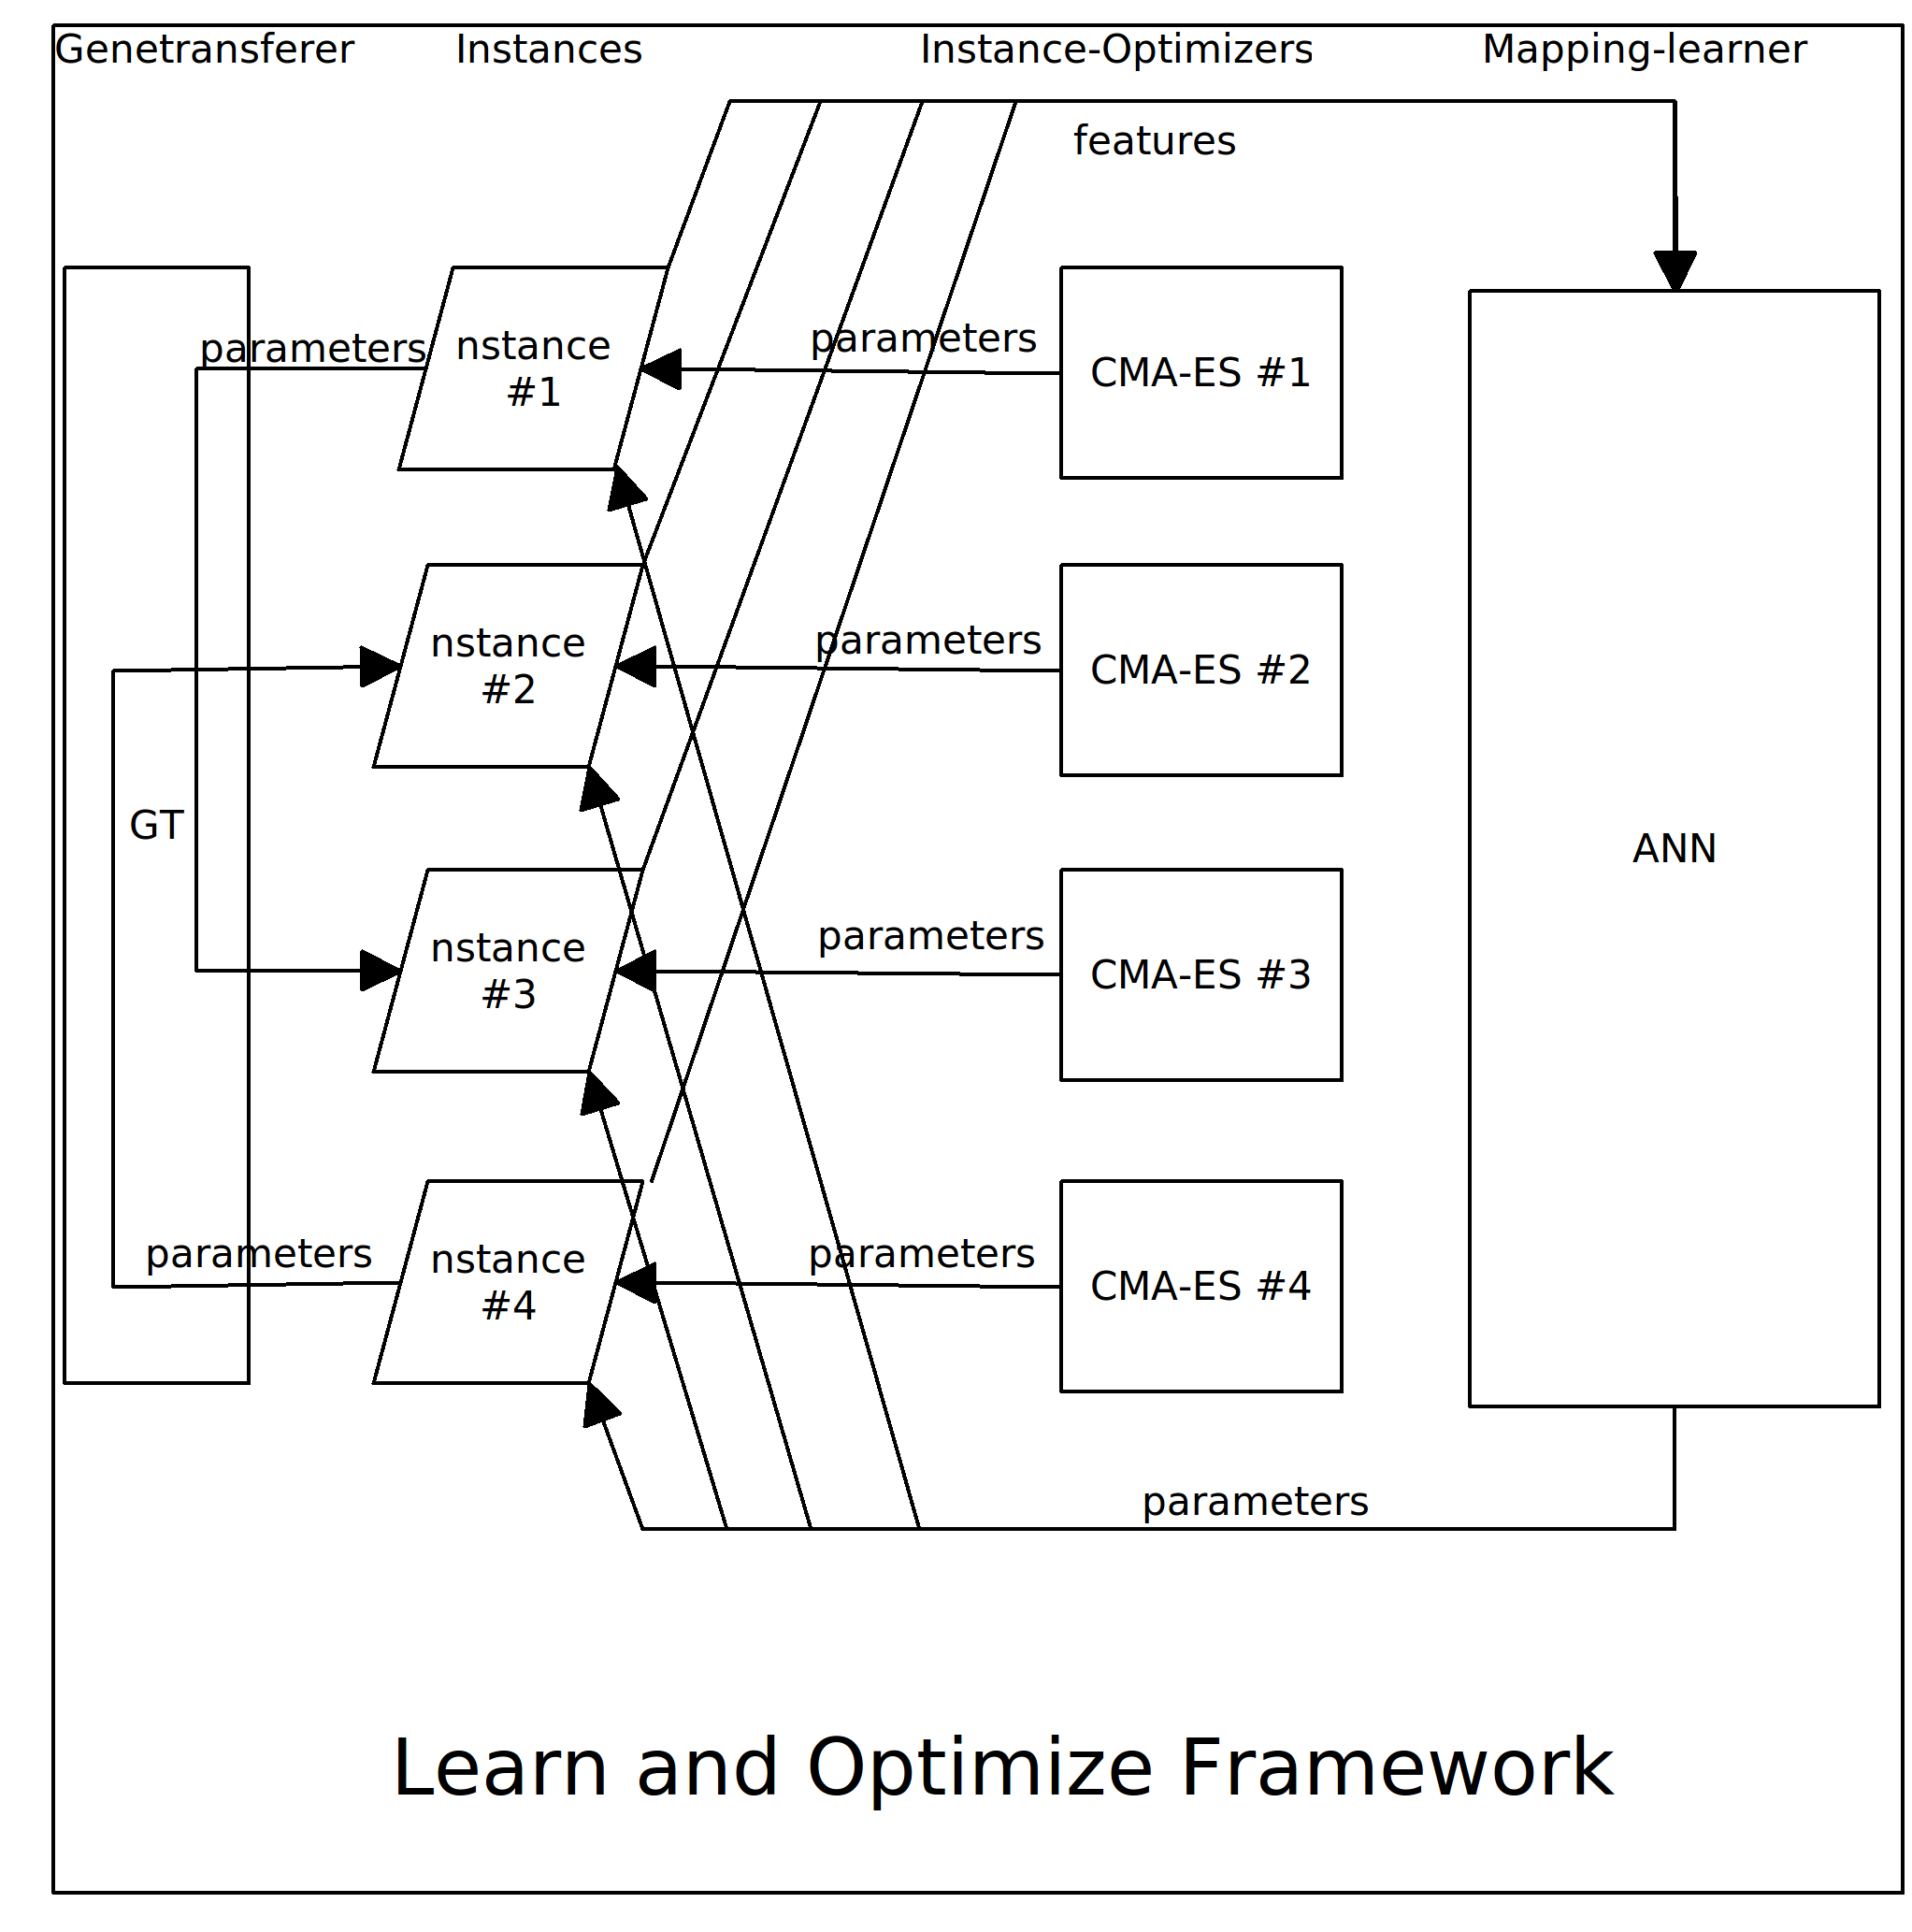
\includegraphics[width=0.4\textwidth]{lao.png}
  \caption{Flowchart of the LaO framework, displaying only 4 instances.}
\label{figure:laoflowchart}
\end{figure}

\begin{table*}[ht] 
\centering
\begin{tabular}{l c c c c c c c}
\hline\hline
Domain & \# of & \# training & \# test &  ANN & quality-ratio & quality-ratio & quality-ratio \\ 
Name & iterations  & instances &  instances &  error & in LaO & ANN on train & ANN on test \\ 
\hline
Freecell& 16 & 108 & 230 & 0.1 & 1.09 & 1.05 & 1.04  \\
Grid & 10 & 55 & 124 & 0.09 & 1.09 & 1.05 & 1.03  \\
Mprime & 8 & 64 & 152 & 0.08 & 1.11 & 1.05 & 1.04   \\
\hline
\end{tabular}
\caption{Results by domains. ANN-error is given as MSE, as returned by FANN. The quality-improvement ratio "in LaO" is that of the best parameter-set found by LaO.}
\label{table:domains}
\end{table*} 

Suppose that we have $n$ features and $m$ parameters (considered to be continuous), and we are doing per-instance parameter tuning on instance $\cal I$ by optimizing the fitness function \begin{math}f_{\cal I}:\mathbf{R}^m\to \mathbf{R} \end{math}, the expected value of DaE executed with parameters \begin{math} p \in \mathbf{R}^m \end{math}. The optimal parameter set is defined by \begin{math} p_{opt}=argmin_p\{f_{\cal I}(p)\} \end{math}. For each instance $\cal I$, consider the set of features: \begin{math} F({\cal I}) \end{math}. We try to learn the mapping from the feature space to the optimal parameter space, which might not be totally unambiguous.

\begin{equation} p: \mathbf{R}^n \to \mathbf{R}^m, p(F)=p_{opt} \end{equation}.	

A multilayer Feed-Forward Artificial Neural Network (ANN) was chosen for the learning of the features-to-parameters mapping. The intermediate models were already used in optimization as in standard surrogate-model based techniques. As an optimizer for each instance a simple yet robust (1+1)-Covariance Matrix Adaptation Evolution Strategy \cite{hansen2001ecj} was chosen. In addition random gene-transfer between instances was developed, transferring to all of the instances with uniform random distribution the so-far best parameter of a different instance. Figure \ref{figure:laoflowchart} shows the LAO framework with the described implementations. The implementation of LaO uses the Shark library \cite{shark08} for CMA-ES and the FANN library for ANN \cite{nissen}. Since DaE is not deterministic, the median of 11 independent runs of DaE with a given parameter-set was computed.



\begin{table}[ht] \small
\centering
\begin{tabular}{l c c c}
\hline\hline
Name & Min & Max & Default \\ 
\hline
Probability of crossover & 0.0 & 1 & 0.8 \\
Probability of mutation & 0.0& 1& 0.2 \\
Rate of mutation add station& 0& 10& 1 \\
Rate of mutation delete station& 0& 10& 3 \\
Rate of mutation add atom& 0& 10& 1 \\
Rate of mutation delete atom& 0& 10& 1 \\
Mean average for mutations& 0.0& 1& 0.8 \\
Time interval radius& 0& 10& 2 \\
Maximum number of stations& 5& 50& 20 \\
Maximum number of nodes& 100& 100 000& 10 000 \\
Population size& 10& 300& 100 \\
Number of offspring & 100& 2 000& 700 \\
\hline
\end{tabular}
\caption{DaE parameters that are controlled by LaO}
\label{table:parameters}
\end{table} 

One iteration of LaO amounts to 5 iterations of CMA-ES, followed by one ANN training and one Genetransferer. The ANN had 3 fully connected layers, the input and hidden layer had both 12 neurons corresponding the number of features. In one iteration of LaO, the ANN was only trained for 50 epochs. After stopping LaO, retraining was made with 300 ANN epochs with the best data, to avoid under-training. The controlled parameters of DaE are described in table \ref{table:parameters}. The feature-set consists of 12 features. The first 6 features are computed from the domain and instance files: number of fluents, goals, predicates, objects and types. One further feature is called mutex-density, which is the number of so-called "mutexes" divided by the number of all fluent-pairs. We also kept 6 less important features: number of lines, words and byte-count of the instance and the domain file.

For evaluation the quality-improvement the quality-ratio metric defined in IPC competitions was used. The baseline is the default parameter-setting. The ratio of the fitness value for the default parameter and the tuned parameter was computed and average was taken over the instances in the train or test-set. 

\begin{equation}Q=\frac{Fitness_{baseline}}{Fitness_{tuned}}\end{equation}

3 sample domains were selected from the Planning and Learning Part of IPC2011: Freecell, Grid, and Mprime. As it can be seen in Table \ref{table:domains}, some quality-gain in training was consistently achieved, but the transfer of this improvement to the ANN-model was only partial, probably because the feature-set is not strong enough. On the other hand, the ANN model generalizes excellently to the the independent test-set. 

\bibliographystyle{abbrv}
\bibliography{gecco2011brendelschoenauer}
\end{document}






